\chapter{Experiments}
\label{ch:intro}

In order to evaluate our extension of ILP, the correlation and lattice, and the different interestingness measures, we
perform a series of experiments on Linked Data.

First, we test our proposed approach on LinkedMDB and DBpedia. We merge both datasets onto a single RDF3X database,
create correlation lattices for the prorperties $budget$ and $runtime$ with categorical relations: $director$,
$writer$, $producer$, $distributor$, $starring$, $country$, and $subject$. We build a pair lattices for each of the 4
interestingness meaures we evaluate: Kullback-Leibler divergence only, Kullback-Leibler combined with support,
Jensen-Shannon combined with support, and support only

Subsequently, we run the ILP with our proposed extension and learn rules with the realtion $country$ as head. We
measure the number of rules with interesting numerical intervals, the runtime spent with their search. It is done for
each of the 4 measures and various different threshold values in order to obtain, and compare their precision recall
graphs. Also we compare their efficiecy by comparing the amount of rules learned per runtime. It is important to point
out that the core-ILP runtime, excluding the search for rules with numerical intervals, is the same for all of them
measures and threshold values. 

Firstly, we compare different measures by building same-sized correlation lattices on the $hasIncome(X,Y)$
relation from the USCensus, then searching for interesting rules with intervals for $Y$ inside the lattice itself as
described in Section~\ref{sec:searchRulesInCL}. The lattices are build by greedily choosing the top-k most interesting
nodes in each level according to the chosen measure, and pruning the rest so that all the lattices have the same
quantity of nodes.

Also, we measure the total time spent for the construction of each lattice as well as the number of interesting rules
found in it. As candidate categorical relations, we chose the 18 shown in Table~\ref{tab:uscensusRelations}. More
details about the categories can be found at the PUMS
Data
Dictionary\footnote{\url{http://www.census.gov/acs/www/Downloads/data_documentation/pums/DataDict/PUMSDataDict05_07.pdf}
}

\begin{table}[h!]
\begin{minipage}{\textwidth}
 \begin{center}
 \caption{Chosen categorical relations from USCensus}
  \begin{tabular}{l l c}
    \toprule
      Name	& Label				& Number of Categories \\
    \midrule
      sex	& Sex				&	2	\\
      st	& State				&	52\footnote{Including Puerto Rico and Washington D.C.}	\\
      racwht	& is White			&	2	\\
      racblk	& is Black			&	2	\\
      racasn	& is Asian			&	2	\\
      qtrbir	& Quarter of Birth		&	4	\\	
      nativity	& born In the US		&	2	\\
      mar	& Marital Status		&	5	\\
      lanp	& Language Spoken at Home	&	104	\\
      esr	& Employment Status		&	6	\\
      dphy	& Physical Difficulty		&	2	\\
      schl	& Educational Level		&	17	\\	
      occp	& Occupation			&	470	\\
      sch	& School Enrollment		&	3	\\
      rel	& Relationship			&	12	\\
      esp	& Employment Status of Parents	&	8	\\
      oc	& Own Child			&	2	\\
    \bottomrule
  \end{tabular}
 \label{tab:uscensusRelations}
 \end{center}
\end{minipage}
\end{table}




Since the USCensus data is completely joined on person entities, and all categorical relations have literals as
constants (usually integer numbers mapped to a set of) of entities 

***Roughly explaining the experiments I did so far, we want to evaluate whether the heuristics are good.
So we use US Census data to build a lattice (for income property) with the limitation of having up to $n$ nodes at each
level. So far I compared the KL-divergence*Support with support only as measures. For every level I sort the nodes by
the measure (nodes with multiple parents will have multiple KL-divergence, in this case I take the maximum one) and try
to join the nodes with highest measures first until $n$ nodes for the next level is reached. In other words, I greedily
build the a lattice with limited number of nodes per level.

After that, I try to extract rules with interesting ranges directly from the lattice and test them against a test
partition. Interesting rules are defined as in \refname{Interesting Rules} with support threshold of 25 examples and
confidence threshold of 0.75. After that, I compare the number of interesting rules learned, the time taken to build the
lattice and the confidence and confidence gain compared to the base rule.

Confidence and confidence gain seem to depend exclusively on the confidence threshold, so they are roughly the same for
both
measures. Processing time is much smaller for the KL-divergence as it doesn't simply focus on huge relations and as
expected, it also presents a greater number of rules with interesting ranges (at least for smaller number of nodes per
level).

Hopefully I'll soon have results from applying the lattice in the core ILP. I managed to overcome some
implementation problems I had when creating the lattice in YAGO.

\begin{figure}
\caption{Lattices with 3 levels}
\centering
\begin{tikzpicture}[scale=1.0]
 \begin{axis}[
	width=15cm, height=10cm,
        xlabel=\textsc{\#Nodes per lattice level},
        ylabel=\textsc{Time to build lattice ($ms$)}
    ]
\addplot coordinates {(5,2165) (10,4337) (15,6723) (20,8860) (30,11969) (40,14626) (50,21288) (60,22329) (70,24577)
(80,25387) (90,27539) (100,30210)};
\addplot coordinates {(5, 235) (10,748) (15, 1317) (20, 1590) (30, 1890) (40, 2482) (50, 3182) (60, 3474) (70, 4020)
(80, 4911) (90,5982) (100,6684)};
\end{axis}
\end{tikzpicture}

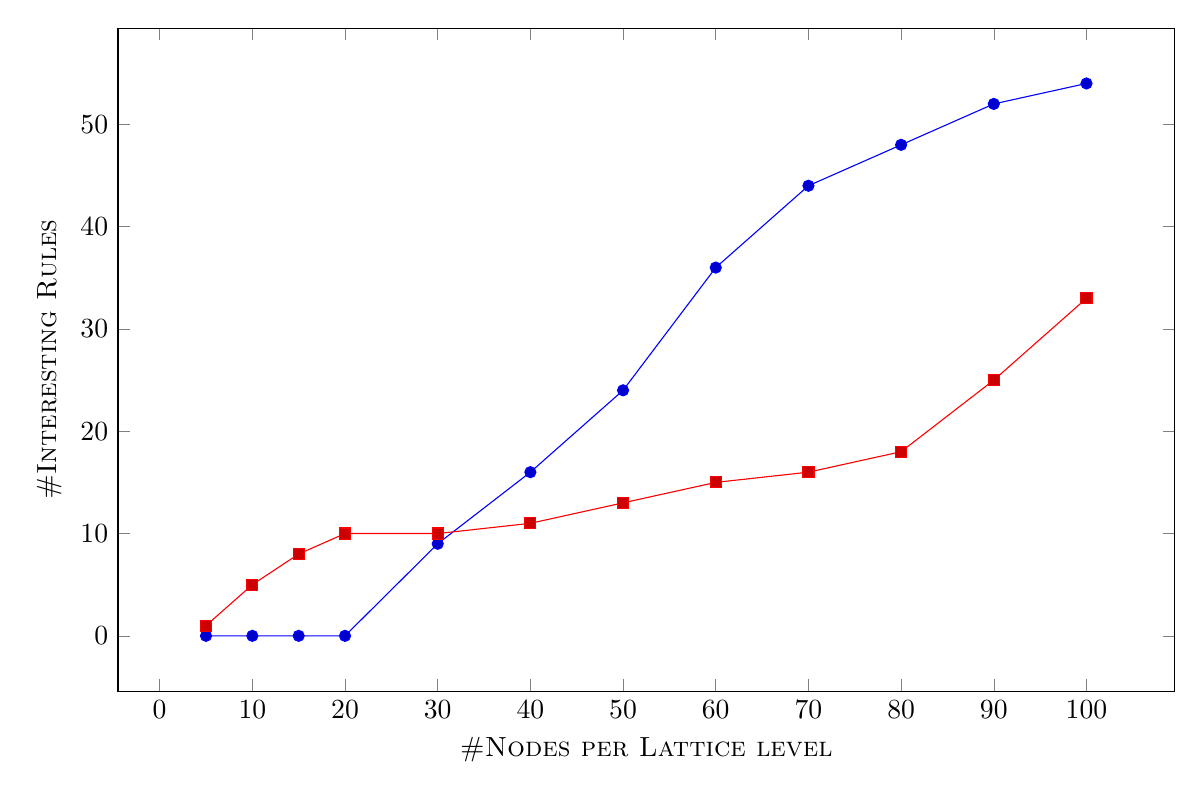
\begin{tikzpicture}[scale=1.0]
 \begin{axis}[
	width=15cm, height=10cm,
        xlabel=\textsc{\#Nodes per Lattice level},
        ylabel=\textsc{\#Interesting Rules}
    ]
\addplot coordinates {(5,0.0) (10,0.0) (15,0.0) (20, 0) (30, 9) (40,16) (50,24) (60,36) (70,44) (80,48) (90,52)
(100,54)};
\addplot coordinates {(5,1.0) (10,5) (15,8) (20,10) (30,10) (40,11) (50,13) (60,15) (70,16) (80,18) (90,25) (100,33)};
\end{axis}
\end{tikzpicture}
\end{figure}

\begin{figure}
 \caption{Lattice with 4 levels}
 \centering
 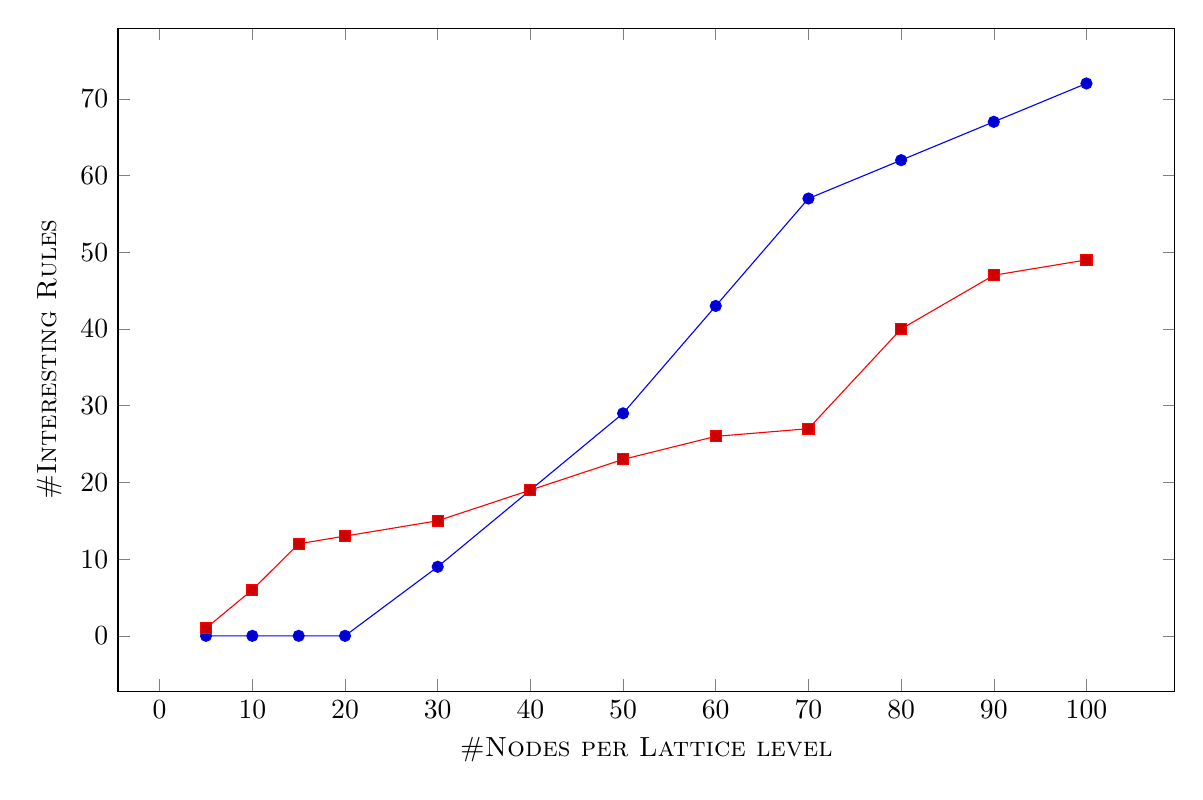
\begin{tikzpicture}[scale=1.0]
  \begin{axis}[
	  width=15cm, height=10cm,
	  xlabel=\textsc{\#Nodes per Lattice level},
	  ylabel=\textsc{\#Interesting Rules}
      ]
  \addplot coordinates {(5,0.0) (10,0.0) (15, 0) (20, 0) (30, 9) (40,19) (50,29) (60,43) (70,57) (80,62) (90,67)
(100,72)};
  %(110,75) (120,79) (130,84) (140,88) (150,94) (200,122) (250,159) (300,178) (350,200) (400,214) (450,231) (500,242)};
  \addplot coordinates {(5,1.0) (10,6) (15,12) (20,13) (30,15) (40,19) (50,23) (60,26) (70,27) (80,40) (90,47)
(100,49)};
  %(110,) (120,) (130,) (140,) (150,) (200,) (250,) (300,) (350,) (400,) (450,) (500,)};
  \end{axis}
  \end{tikzpicture}
  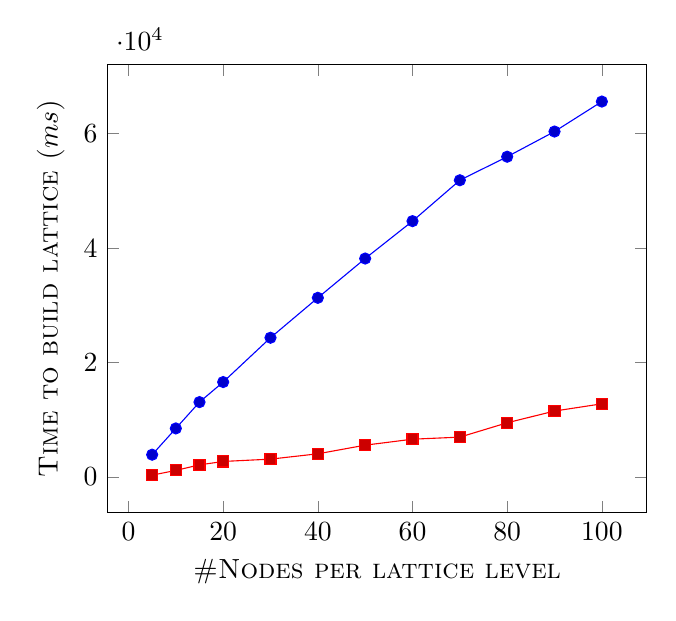
\begin{tikzpicture}[scale=1.0]
  \begin{axis}[
	  xlabel=\textsc{\#Nodes per lattice level},
	  ylabel=\textsc{Time to build lattice ($ms$)}
      ]
  \addplot coordinates {(5,3905) (10,8496) (15,13097) (20,16601) (30,24348) (40,31322) (50,38189) (60,44724) (70,51869)
  (80,55981) (90,60382) (100,65622)};
% (110,75) (120,79) (130,84) (140,88) (150,94) (200,122) (250,159) (300,178)  (350,200) (400,214) (450,231) (500,242)};
  \addplot coordinates {(5, 330) (10,1161) (15, 2128) (20, 2722) (30, 3130) (40, 4060) (50, 5571) (60, 6613) (70, 6976)
  (80, 9483) (90,11534) (100,12795)};
% (110,) (120,) (130,) (140,) (150,) (200,) (250,) (300,) (350,) (400,) (450,) (500,)};
  \end{axis}
  \end{tikzpicture}
\end{figure}

\begin{figure}
 \caption{Precision - Recall }
 \centering
 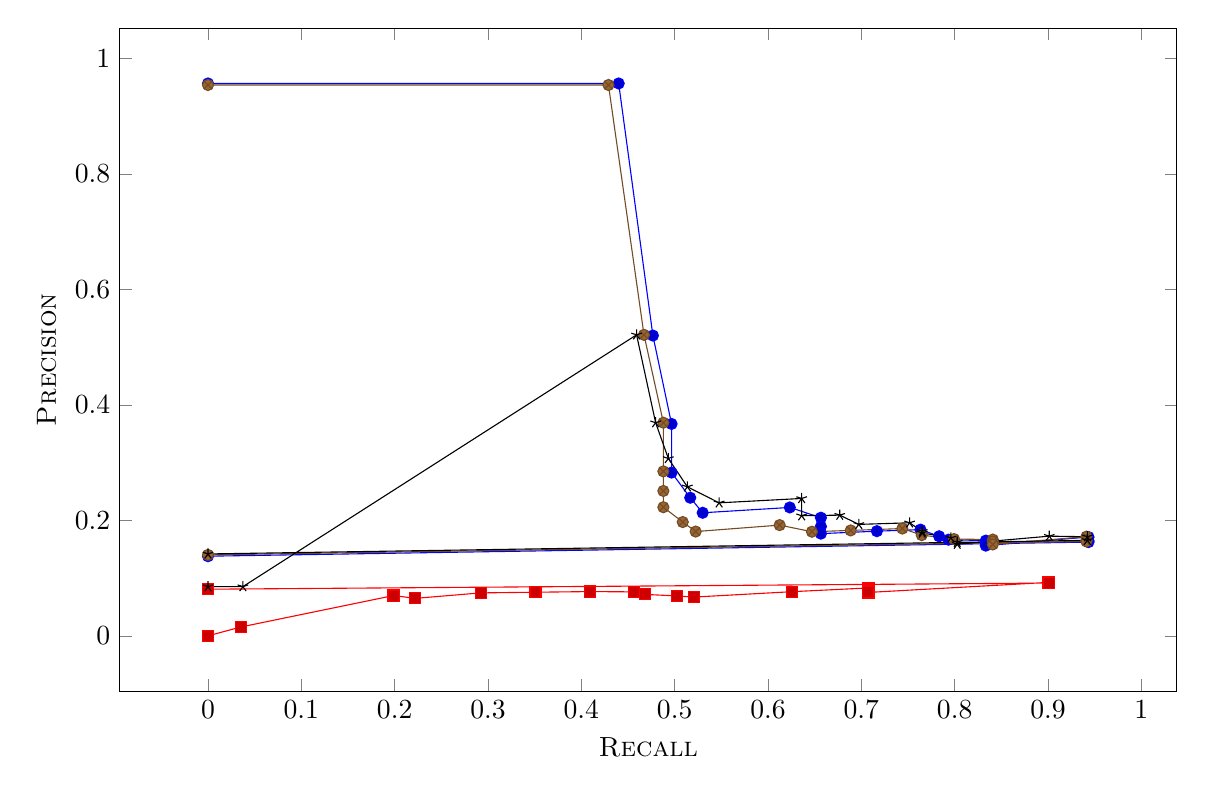
\begin{tikzpicture}[scale=1.0]
  \begin{axis}[
  	  width=15cm, height=10cm,
	  xlabel=\textsc{Recall},
	  ylabel=\textsc{Precision}
      ]
  \addplot coordinates {(0,0.9565217) (0.44,0.9565217) (0.4766667,0.52) (0.4966667,0.3669951) 
(0.4966667,0.2827325) (0.5166667,0.2391975) (0.53,0.2131367) (0.6233333,0.2223543) (0.6566667,0.2045691)
 (0.6566667,0.1894231) (0.6566667,0.1769991) (0.7166666,0.1812816) (0.7633333,0.1839358) (0.7833334,0.1724138)
 (0.7933334,0.1665500) (0.8333333,0.1649076) (0.8333333,0.1612903) (0.8333333,0.15625) (0.9433333,0.1711004) 
 (0.9433333,0.1644393) (0.9433333,0.1623637) (0,0.1379310)};
  \addplot coordinates {(0,0) (0,0) (0,0) (0,0) (0.03508772,0.01530612) (0.1988304,0.0698152) 
  (0.2222222,0.06495727) (0.2923977,0.07440476) (0.3508772,0.07556675) (0.4093567,0.07667032) (0.4561403,0.07617188)
(0.4678363,0.07181329) (0.502924,0.06907631) (0.5204678,0.06711916) (0.625731,0.0764832) (0.7076023,0.0829904)
(0.7076023,0.0810992) (0.7076023,0.07846952) (0.7076023,0.07520199) (0.9005848,0.09260373)
 (0.9005848,0.09139466) (0,0.08077468)};
  \addplot coordinates { (0,0.9538462) (0.4290657,0.9538462) (0.467128,0.5212355) (0.4878893,0.3691100)
(0.4878893,0.2848485) (0.4878893,0.2508897) (0.4878893,0.2227488) (0.5086505,0.1970509) (0.5224913,0.180622)
(0.6124567,0.1917660) (0.6470588,0.1803279) (0.6885813,0.1825688) (0.7439446,0.1858254) (0.7647059,0.1744278)
(0.799308,0.1676343) (0.8408305,0.1667810) (0.8408305,0.1631968) (0.8408305,0.1583062) (0.9411765,0.1718256)
(0.9411765,0.1654501) (0.9411765,0.1634615) (0,0.1401552)};
  \addplot coordinates {(0,0.08527132) (0.03741496,0.08527132) (0.4591837,0.5212355) (0.4795918,0.3691100)
(0.4931973,0.3072034)
(0.5136054,0.2581197) (0.547619,0.2303290) (0.6360544,0.2379135) (0.6360544,0.2080089) (0.6768708,0.2090336)
(0.6972789,0.193032) (0.7517007,0.1957484) (0.7653061,0.1810137) (0.7653061,0.1781473) (0.7959183,0.1696882)
(0.8027211,0.1621993) (0.8027211,0.1587088) (0.9013606,0.1726384) (0.9421769,0.1716233) (0.9421769,0.1653731)
(0,0.1418234)};
  \end{axis}
  \end{tikzpicture}
\end{figure}

\begin{figure}
 \caption{Runtime-LearnedRules}
 \centering
 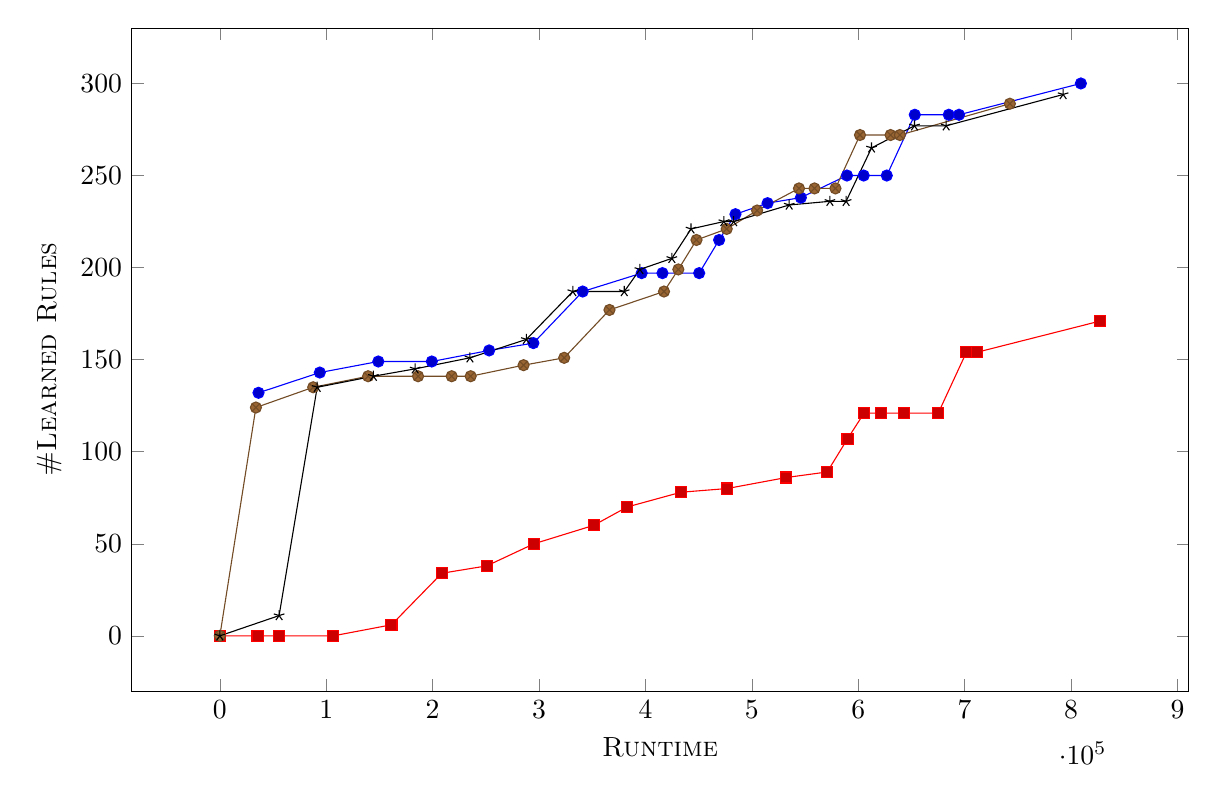
\begin{tikzpicture}[scale=1.0]
  \begin{axis}[
  	  width=15cm, height=10cm,
	  xlabel=\textsc{Runtime},
	  ylabel=\textsc{\#Learned Rules}
      ]
  \addplot coordinates { (36343,132) (93944,143) (148944,149) (199223,149) (253104,155) (294678,159) (341024,187)
(396459,197) (416000,197) (450504,197) (469231,215) (484591,229) (514785,235) (546069,238) (589417,250) (605128,250)
(626821,250) (653140,283) (685085,283) (694687,283) (809238,300)};
  \addplot coordinates {(0.0,0.0) (35466,0.0) (55421,0.0) (106586,0.0) (161302,6) (208629,34) (250863,38) (295212,50)
(351300,60)
(382899,70) (433423,78) (476677,80) (532442,86) (570818,89) (589925,107) (605518,121) (621333,121) (643190,121)
(675208,121) (701631,154) (711515,154) (827520,171)};
  \addplot coordinates {(0.0,0.0) (33892,124) (87747,135) (139353,141) (186294,141) (217893,141) (235750,141)
(285443,147)
(323626,151) (366197,177) (417438,187) (430932,199) (447970,215) (476371,221) (504948,231) (544307,243) (558897,243)
(578569,243) (601647,272) (630384,272) (639120,272) (742514,289)};
  \addplot coordinates {(0.0,0.0) (55709,11) (91488,135) (144319,141) (183567,145) (235053,151) (288040,161)
(331747,187)
(380080,187) (394814,199)
(424827,205) (442860,221) (473691,225) (482918,225) (535099,234) (573386,236) (588600,236) (612505,265) (652833,277)
(682636,277) (792557,294)};
  \end{axis}
  \end{tikzpicture}
\end{figure}


\subsection{Example of Rules Learned}

We selected a couple of interesting rules learned with our approach in order to illustrate the kind of results we
obtain. On LinkedMDB, for example, we learned that films in English with Canadian director, and low budget are
significantly more likely to be also Canadian than those with higher budget. The base rule shown below has
confidence $0.36$:

$country(X,canada)$ :- $director(X,Z),bornIn(Z,canada),language(X,english),budget(X,Y)$

When we refine this rule, we find an interval with confidence $0.83$:

$country(X,canada)$ :- $director(X,Z),bornIn(Z,canada),language(X,english),budget(X,Y),Y\leq 80000$

Another interesting example reveals that films written by a spouse of Fritz Lang (in this case, Thea von
Harbou, who was an actress, writer, and director), and which have long runtime are more likely to have been directed by
Fritz Lang than those with shorter runtime. The base rule has confidence $0.6$:

$director(X,fritzLang)$ :- $writer(A,D),spouse(D,fritzLang),runtime(X,Y)$

And the refined rule has confidence $0.82$:

$director(X,fritzLang)$ :- $writer(A,D),spouse(D,fritzLang),runtime(X,Y),Y\geq 6800s$

Other examples of interesting rules learned are shown in Table~\ref{tab:mdbRuleExamples}.

\begin{table}[h!]
\begin{minipage}{\textwidth}
 \begin{center}
 \caption{Interesting rules with numerical intervals learned from DBpedia}
  \begin{tabular}{ >{\emph}r >{\raggedright}p{7cm} | c | c }
    \toprule
      & Refined Rule				& Conf 	& Gain \\
    \midrule
      country(X,canada) :-&director(X,Z), bornIn(Z,canada), language(X,english), budget(X,Y), Y$\leq 80000$ &
      0.83	& 0.36 \\ \hline
      director(X,fritzLang) :-&writer(X,Z), spouse(Z,fritzLang), runtime(X,Y), Y$\geq 6800s$ & 
      0.82	& 0.37 \\ \hline
      writer(X,sylvesterStallone) :-&starring(X,sylvesterStallone), subject(X,englishLanguageFilms),
      budget(X,Y), Y$\in [6M,31M]$ &
      0.89	& 0.48 \\ \hline
      producer(X,clintEastwood) :-&director(X,clintEastwood), starring(X,clintEastwood),
      subject(X,englishLanguageFilms), budget(X,Y), Y$\geq 13M$ &
      1.00	& 0.73 \\ \hline
      starring(X,clintEastwood) :- &budget(X,Y), director(X,clintEastwood), starring(A,clintEastwood), 
      subject(A,englishLanguageFilms), Y$\in [930K,25M]$&
      0.82	& 0.56 \\ \hline
      starring(X,Z) :-&writer(X,Z), country(X,uk), distributor(X,bbc),r untime(X,Y), Y$\leq 4080s$ &
      0.9	& 0.53 \\ \hline

    \bottomrule
  \end{tabular}
 \label{tab:mdbRuleExamples}
 \end{center}
\end{minipage}
\end{table}


On the

\begin{table}[h!]
\begin{minipage}{\textwidth}
 \begin{center}
 \caption{Interesting rules with numerical intervals learned from USCensus}
  \begin{tabular}{ >{\textit}r >{\raggedright}p{7cm} | c | c }
    \toprule
      & Refined Rule				& Conf 	& Gain \\
    \midrule

    \bottomrule
  \end{tabular}
 \label{tab:uscensusRuleExamples}
 \end{center}
\end{minipage}
\end{table}



\begin{figure}
 \caption{Precision - Recall }
 \centering
 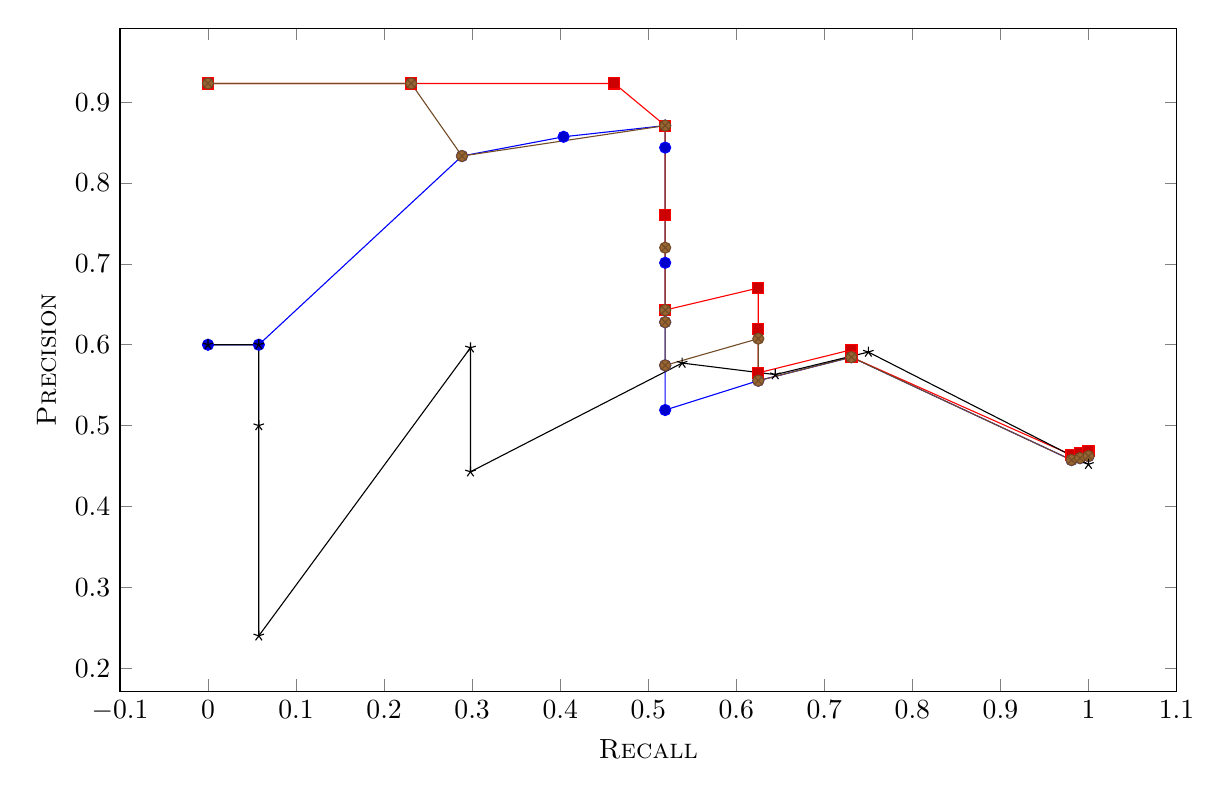
\begin{tikzpicture}[scale=1.0]
  \begin{axis}[
  	  width=15cm, height=10cm,
	  xlabel=\textsc{Recall},
	  ylabel=\textsc{Precision}
      ]
  \addplot coordinates {(0.0,0.6) (0.05769231,0.6) (0.2884615,0.8333333) (0.4038461,0.8571429) (0.5192308
, 0.8709678) (0.5192308,0.84375) (0.5192308,0.7012987) (0.5192308,0.627907) (0.5192308,0.5744681) (
0.5192308,0.5192308) (0.625,0.5555556) (0.7307692,0.5846154) (0.9807692,0.4573991) (0.9903846 ,
0.4598214) (1.0,0.4622222)};
  \addplot coordinates {(0.0,0.9230769) (0.2307692,0.9230769) (0.4615385,0.9230769) (0.5192308,0.8709678)
(0.5192308,0.7605634) (0.5192308,0.6428571) (0.625,0.6701031) (0.625,0.6190476) (0.625,0.5652174) (
0.7307692,0.59375) (0.7307692,0.5846154) (0.9807692,0.4636364) (0.9903846,0.4660633) (1.0,0.4684685)};
  \addplot coordinates { (0.0,0.9230769) (0.2307692,0.9230769) (0.2884615,0.8333333) (0.5192308,0.8709678)
(0.5192308,0.72) (0.5192308,0.6428571) (0.5192308,0.627907) (0.5192308,0.5744681) (0.625,0.6074766)
(0.625,0.5555556) (0.7307692,0.5846154) (0.9807692,0.4573991) (0.9903846,0.4598214) (1.0,0.4622222)};
  \addplot coordinates {(0.0,0.6) (0.05769231,0.6) (0.05769231,0.5) (0.05769231,0.24) (0.2980769 ,
0.5961539) (0.2980769,0.4428571) (0.5384616,0.5773196) (0.6442308,0.5630252) (0.75,0.5909091) (1 ,
0.4521739)};
  \end{axis}
  \end{tikzpicture}
\end{figure}


\begin{figure}
%\begin{minipage}{1\linewidth}\centering
 \caption{Runtime-LearnedRules}
 \centering
 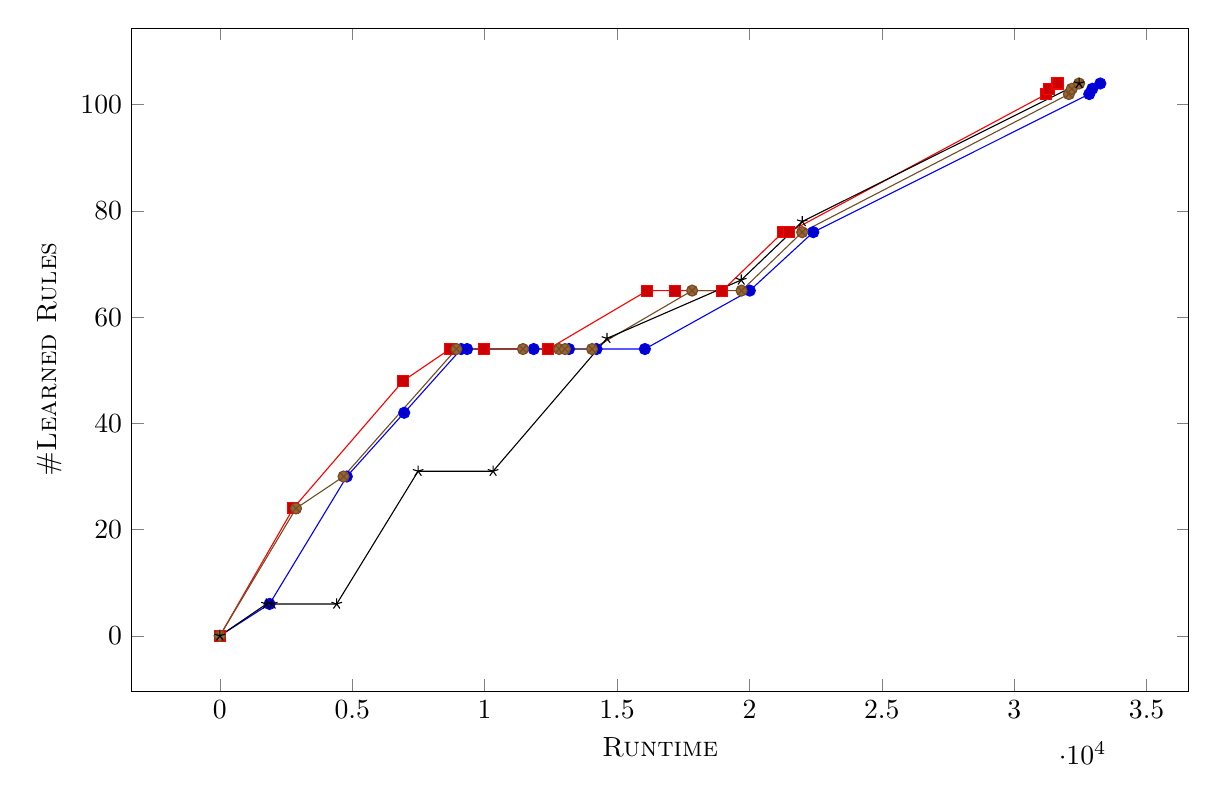
\begin{tikzpicture}
  \begin{axis}[
	  width=15cm, height=10cm,
	  xlabel=\textsc{Runtime},
	  ylabel=\textsc{\#Learned Rules}
      ]
  \addplot coordinates {(0.0,0.0) (1877,6) (4795,30) (6962,42) (9116,54) (9337,54) (11852,54) (
13187,54) (14225,54) (16052,54) (20014,65) (22411,76) (32833,102) (32949,103) (33251,104
)};
  \addplot coordinates {(0.0,0.0) (2772,24) (6923,48) (8690,54) (9977,54) (12400,54) (16145,65)
(17187,65) (18979,65) (21270,76) (21483,76) (31215,102) (31324,103) (31637,104)};
  \addplot coordinates {(0.0,0.0) (2877,24) (4672,30) (8934,54) (11447,54) (12813,54) (13033,54)
(14057,54) (17836,65) (19703,65) (21991,76) (32064,102) (32173,103) (32449,104)};
  \addplot coordinates { (0.0,0.0) (1762,6) (1976,6) (4413,6) (7488,31) (10319,31) (14620,56) (
19691,67) (21995,78) (32452,104)};
  \end{axis}
  \end{tikzpicture}
 % \end{minipage}
\end{figure}




